%%%%%%%%%%%%%%%%%%%%%%%%%%%%%%%%%%%%%%%%%%%%%%%%%%%%%%%%%%%%%%%%%%%%%%%%%%%%%%%%
%%%%%%%%%%%%%%%%%%%%%%%%%%%%%%%%%%%%%%%%%%%%%%%%%%%%%%%%%%%%%%%%%%%%%%%%%%%%%%%%
%%                                                                            %%
%% thesistemplate.tex version 4.10 (2025/06/30)                               %%
%% The LaTeX template file to be used with the aaltothesis.sty (version 4.10) %%
%% style file.                                                                %%
%% This package requires pdfx.sty v. 1.5.84 (2017/05/18) or newer.            %%
%%                                                                            %%
%% This is licensed under the terms of the MIT license below.                 %%
%%                                                                            %%
%% Written by Luis R.J. Costa.                                                %%
%% Currently developed at Teacher services, Learning Services of Aalto        %%
%% University by Luis R.J. Costa since May 2019.                              %%
%%                                                                            %%
%% Copyright 2017-2025 aaltothesis.cls by Luis R.J. Costa,                    %%
%% luis.costa@aalto.fi.                                                       %%
%% Copyright 2017-2018 Swedish translations in aaltothesis.cls by Elisabeth   %%
%% Nyberg and Henrik Wallén henrik.wallen@aalto.fi.                           %%
%% Copyright 2017-2018 Finnish documentation in the template opinnatepohja.tex%%
%% by Perttu Puska, perttu.puska@aalto.fi, and Luis R.J. Costa.               %%
%% Finnish documentation in the template opinnatepohja.tex translated from    %%
%% the English template documentation.                                        %%
%% Copyright 2025 English template thesistemplate.tex by Luis R.J. Costa,     %%
%% Maurice Forget, Henrik Wallén.                                             %%
%% Copyright 2018-2025 Swedish template kandidatarbetsbotten.tex by Henrik    %%
%% Wallen.                                                                    %%
%%                                                                            %%
%% Permission is hereby granted, free of charge, to any person obtaining a    %%
%% copy of this software and associated documentation files (the "Software"), %%
%% to deal in the Software without restriction, including without limitation  %%
%% the rights to use, copy, modify, merge, publish, distribute, sublicense,   %%
%% and/or sell copies of the Software, and to permit persons to whom the      %%
%% Software is furnished to do so, subject to the following conditions:       %%
%% The above copyright notice and this permission notice shall be included in %%
%% all copies or substantial portions of the Software.                        %%
%% THE SOFTWARE IS PROVIDED "AS IS", WITHOUT WARRANTY OF ANY KIND, EXPRESS OR %%
%% IMPLIED, INCLUDING BUT NOT LIMITED TO THE WARRANTIES OF MERCHANTABILITY,   %%
%% FITNESS FOR A PARTICULAR PURPOSE AND NONINFRINGEMENT. IN NO EVENT SHALL    %%
%% THE AUTHORS OR COPYRIGHT HOLDERS BE LIABLE FOR ANY CLAIM, DAMAGES OR OTHER %%
%% LIABILITY, WHETHER IN AN ACTION OF CONTRACT, TORT OR OTHERWISE, ARISING    %%
%% FROM, OUT OF OR IN CONNECTION WITH THE SOFTWARE OR THE USE OR OTHER        %%
%% DEALINGS IN THE SOFTWARE.                                                  %%
%%                                                                            %%
%%                                                                            %%
%%%%%%%%%%%%%%%%%%%%%%%%%%%%%%%%%%%%%%%%%%%%%%%%%%%%%%%%%%%%%%%%%%%%%%%%%%%%%%%%
%%                                                                            %%
%%                                                                            %%
%% An example for writting your thesis using LaTeX                            %%
%% Original version and development work by Luis Costa, changes to the text   %% 
%% in the Finnish template by Perttu Puska.                                   %%
%% Support for Swedish added 15092014                                         %%
%% PDF/A-b support added on 15092017                                          %%
%% PDF/A-2 support added on 24042018                                          %%
%% Layout design and typesettin changed 15072021                              %%
%%                                                                            %%
%% This example consists of the files                                         %%
%%       thesistemplate.tex (version 4.10) (for text in English)              %%
%%       opinnaytepohja.tex (version 4.10) (for text in Finnish)              %%
%%       kandidatarbetsbotten.tex (version 1.20) (for text in Swedish)        %%
%%       thesistemplate_short.tex (version 4.10) (abridged for text in        %%
%%                                                English)                    %%
%%       aaltothesis.cls (version 4.10)                                       %%
%%       linediagram.pdf (graphics file)                                      %%
%%       curves.pdf      (graphics file)                                      %%
%%       ledspole.jpg    (graphics file)                                      %%
%%                                                                            %%
%%                                                                            %%
%% Typeset in Linux with                                                      %%
%% pdflatex: (recommended method)                                             %%
%%             $ pdflatex thesistemplate                                      %%
%%             $ pdflatex thesistemplate                                      %%
%%                                                                            %%
%%   The result is the file thesistemplate.pdf that is PDF/A compliant, if    %%
%%   you have chosen the proper \documenclass options (see comments below)    %%
%%   and your included graphics files have no problems.                       %%
%%                                                                            %%
%%                                                                            %%
%% Explanatory comments in this example begin with the characters %%, and     %%
%% changes that the user can make with the character %                        %%
%%                                                                            %%
%%%%%%%%%%%%%%%%%%%%%%%%%%%%%%%%%%%%%%%%%%%%%%%%%%%%%%%%%%%%%%%%%%%%%%%%%%%%%%%%
%%%%%%%%%%%%%%%%%%%%%%%%%%%%%%%%%%%%%%%%%%%%%%%%%%%%%%%%%%%%%%%%%%%%%%%%%%%%%%%%
%%
%% WHAT is PDF/A
%%
%% PDF/A is the ISO-standardized version of the pdf. The standard's goal is to
%% ensure that he file is reproducable even after a long time. PDF/A differs
%% from pdf in that it allows only those pdf features that support long-term
%% archiving of a file. For example, PDF/A requires that all used fonts are
%% embedded in the file, whereas a normal pdf can contain only a link to the
%% fonts in the system of the reader of the file. PDF/A also requires, among
%% other things, data on colour definition and the encryption used.
%% Currently three PDF/A standards exist:
%% PDF/A-1: based on PDF 1.4, standard ISO19005-1, published in 2005.
%%          Includes all the requirements essential for long-term archiving.
%% PDF/A-2: based on PDF 1.7, standard ISO19005-2, published in 2011.
%%          In addition to the above, it supports embedding of OpenType fonts,
%%          transparency in the colour definition and digital signatures.
%% PDF/A-3: based on PDF 1.7, standard ISO19005-3, published in 2012.
%%          Differs from the above only in that it allows embedding of files in
%%          any format (e.g., xml, csv, cad, spreadsheet or wordprocessing
%%          formats) into the pdf file.
%% PDF/A-4: based on PDF 2.0, standard ISO19005-4, published in November 2020.
%%
%% PDF/A-1 files are not necessarily PDF/A-2 -compatible and PDF/A-2 are not
%% necessarily PDF/A-1 -compatible.
%% Standards PDF/A-1, PDF/A-2 and PDF/A-3 have two levels:
%% b: (basic) requires that the visual appearance of the document is reliably
%%    reproduceable.
%% a (accessible) in addition to the b-level requirements, specifies how
%%   accessible the pdf file is to assistive software, say, for the physically
%%   impaired.
%% The PDF/A-4 standard does not have additional levels like in the earlier
%% standards.
%% For more details on PDF/A, see, e.g., 
%% https://www.loc.gov/preservation/digital/formats/fdd/fdd000318.shtml or
%% https://www.pdfa.org/resource/iso-19005-pdfa/
%%
%%
%% WHICH PDF/A standard should my thesis conform to?
%%
%% Either to the PDF/A-2b or the PDF/A-1b standard. If all the figures and
%% graphs used in thesis work do not require transparency features, use either
%% PDF/A-1b or PFDF/A-2b. If you have figures with transparency
%% characteristics, use the PDF/A-2b standard. However, drawing applications
%% often use the transparency parameter, setting it to zero, to specify opacity
%% and get the basic 2-D visualisation. As a result, validation of PDF/A-1b
%% will fail. Use PDF/A-2b if PDF/A-1b validation fails.
%% Do not use the PDF/A-3b standard for your thesis.
%% The font to be used are specified in this templatenand they should not be
%% changed. In addition to not adhering to Aalto's visual guidelines, you may
%% have difficulties in producing a PDF/A-compliant PDF.
%%
%%
%% Validate your PDF/A file at https://www.pdf-online.com/osa/validate.aspx
%%
%%
%% WHAT graphics format can I use to produce my PDF/A compliant file?
%%
%% When using pdflatex to compile your work, favour the use of pdf, but you can
%% use the jpg or png format especially for photographs. You will have PDF/A 
%% compliance problems with figures in pdf if the fonts are not embedded in the
%% pdf file.
%% If you choose to use latex to compile your work, the only acceptable file
%% format for your figure is eps. DO NOT use the ps format for your figures.
%%
%% USE one of the following three \documentclass set-ups:
%% * the first when using pdflatex to directly typeset your document in the
%%   chosen pdf/a format for online publishing (centred page layout),
%% * the second for one-sided printing your thesis with the layout (wide left 
%%   margin), or
%% * the third for two-sided printing.
%%
\documentclass[english, 12pt, a4paper, elec, utf8, a-2b, online]{aaltothesis}
%\documentclass[english, 12pt, a4paper, elec, utf8, a-2b, print]{aaltothesis}
%\documentclass[english, 12pt, a4paper, elec, utf8, a-2b, print, twoside]{aaltothesis}

%% Use the following options in the \documentclass macro above:
%% your school: arts, biz, chem, elec, eng, sci
%% the character encoding scheme used by your editor: utf8, latin1
%% thesis language: english, finnish, swedish
%% make an archiveable PDF/A-1b or PDF/A-2b compliant file: a-1b, a-2b
%%                    (with pdflatex, a normal pdf containing metadata is
%%                     produced without the a-*b option)
%% typset for online document or print on paper: online, print
%%        online: typeset in symmetric layout and blue hypertext for online
%%                publishing
%%        print: typeset in a symmetric layout and black hypertext for printing
%%               on paper
%%          two-side printing: twoside (default is one-sided printing)
%%               typeset in a wide margin on the binding side of the page and
%%               black hypertext. Use with print only.
%%

%% Use one of these if you write in Finnish (or use the Finnish template
%% opinnaytepohja.tex)
%\documentclass[finnish, 12pt, a4paper, elec, utf8, a-1b, online]{aaltothesis}
%\documentclass[finnish, 12pt, a4paper, elec, utf8, a-1b, print]{aaltothesis}
%\documentclass[finnish, 12pt, a4paper, elec, utf8, a-1b, print, twoside]{aaltothesis}

%% Use one of these if you write in Swedish (or use the Swedish template
%% kandidatarbetsbotten.tex)
%\documentclass[swedish, 12pt, a4paper, elec, utf8, a-2b, online]{aaltothesis}
%\documentclass[swedish, 12pt, a4paper, elec, utf8, a-2b]{aaltothesis}
%\documentclass[swedish, 12pt, a4paper, elec, dvips, online]{aaltothesis}

%% FOR USERS OF AMS PACKAGES:
%% * newtxmath used in this template loads amsmath, so
%%   you needn't load it. If you want to use options in amsmath, load it here, 
%%   before \setupthesisfonts below to pass the options to amsmath.
%% * If you want to use amsthm, load it here before \setupthesisfonts to avoid
%%   a clash with newtxmath.
%% * If using amsmath with options and you want to use amsthm, load amsthms
%%   after amsmath, as described in the amsthm documentation.
%% * Don't use amsbsym or amsfonts. The symbols [and macros] there are defined in
%%   newtxmath and so clash if used.
%\usepackage[options]{amsmath}
%\usepackage{amsthm}

%% DO NOT MOVE OR REMOVE \setupthesisfonts
\setupthesisfonts

%%
%% Add here the packges you need
%%
\usepackage{graphicx}


%% For tables that span multiple pages; used to split a paraphrasing example in
%% the appendix. If you don't need it, remove it.
\usepackage{longtable}

%% A package for generating Creative Commons copyright terms. If you don't use
%% the CC copyright terms, remove it, since otherwise undesired information may
%% be added to this document's metadata.
\usepackage[type={CC}, modifier={by-nc-sa}, version={4.0}]{doclicense}
%% Find below three examples for typesetting the CC license notice.

\usepackage[
backend=biber,
style=numeric-comp, % citations and references are numerical (Vancouver, IEEE)
sorting=none, % cited reference is first in the bibliography followed by all 
              % references in the database references.bib
firstinits=true, % show initial of first name in bibliography
urldate=long % date is expressed as Month dd, yyyy
]{biblatex}
\addbibresource{thesisreferences.bib}

%% Edit to conform to your degree programme
%% Capitalise the words in the name of the degree programme: it's a name
\degreeprogram{Computer, Communication and Information Sciences}
%%

%% Your major
%%
\major{Communications Engineering}
%%

%% Choose one of the three below
%%
%\univdegree{BSc}
\univdegree{MSc}
%\univdegree{Lic}
%%

%% Your name (self explanatory...)
%%
\thesisauthor{David Enberg}
%%

%% Your thesis title and possible subtitle comes here and possibly, again,
%% together with the Finnish or Swedish abstract. Do not hyphenate the title
%% (and subtitle), and avoid writing too long a title. Should LaTeX typeset a
%% long title (and/or subtitle) unsatisfactorily, you might have to force a
%% linebreak using the \\ control characters. In this case...
%% * Remember, the title should not be hyphenated!
%% * A possible 'and' in the title should not be the last word in the line; it
%%   begins the next line.
%% * Specify the title (and/or subtitle) again without the linebreak characters
%%   in the optional argument in box brackets. This is done because the title
%%   is part of the metadata in the pdf/a file, and the metadata cannot contain
%%   linebreaks.
%%
\thesistitle{Performance of Server Message Block implementations over QUIC}
%\thesistitle[Title of the thesis]{Title of\\ the thesis}
%%
%% Either remove or leave \thesissubtitle{} empty if you don't use it
%%
\thesissubtitle{}
%\thesissubtitle[Subtitle of the thesis]{Subtitle of\\ the thesis}
%\thesissubtitle{}

%%
\place{Espoo}
%%

%% The date for the bachelor's thesis is the day it is presented
%%
\date{24 November 2025}
%%

%% Thesis supervisor
%% Note the "\" character in the title after the period and before the space
%% and the following character string.
%% This is because the period is not the end of a sentence after which a
%% slightly longer space follows, but what is desired is a regular interword
%% space.
%%
\supervisor{PhD Pasi Sarolahti}
%%

%% Advisor(s)---two at the most---of the thesis. Check with your supervisor how
%% many official advisors you can have.
%%
\advisor{Bastian Shajit (MSc)}
%%

%% If you do your thesis work in a company of other institute, give the name of
%% the company or instution here. Otherwise, leave the macro empty, comment it
%% out, or remove it. This will remove this field from the abstract page.
%%
\collaborativepartner{Tuxera Oy}
%%

%% Aaltologo: syntax:
%% \uselogo{?|!|'|aalto?|aalto!|aalto'|<empty>}
%% The logo language is set to be the same as the thesis language.
%%
%\uselogo{?}
%\uselogo{!}
\uselogo{'}
%\uselogo{aalto?}
%\uselogo{aalto!}
%\uselogo{aalto'}
%\uselogo{}
%%

%%%%%%%%%%%%%%%%%%               COPYRIGHT TEXT               %%%%%%%%%%%%%%%%%%
%%%%%%%%%%%%%%%%%%%%%%%%%%%%%%%%%%%%%%%%%%%%%%%%%%%%%%%%%%%%%%%%%%%%%%%%%%%%%%%%

%% Copyright of a work is with the creator/author of the work regardless of
%% whether the copyright mark is explicitly in the work or not. You may, if you
%% wish---we encourage you to do so---publish your work under a Creative
%% Commons license (see creativecommons.org), in which case the license text
%% must be visible in the work. Write here the copyright text you want using the
%% macro \copyrighttext, which writes the text into the metadata of the pdf file
%% as well.
%%
%% Syntax:
%% \copyrigthtext{metadata text}{text visible on the page}
%%
%% CHOOSE ONE OF THE COPYRIGHT NOTICE STYLES BELOW.
%% IF USING THE CC TERMS, CHOOSE THE LICENSE YOU WANT TO USE.
%% The different CC licenses are listed at 
%% https://creativecommons.org/about/cclicenses/.
%% If you use the icons from the doclicense.sty package, add the package above
%% (\usepackage{doclicense}).
%% IMPORTANT NOTE!! Manually write the CC text in the \copyrighttext metadata
%% text field.
%%
%% NOTE: In the macros below, the text written in the metadata must have a
%% \noexpand macro before the \copyright special character. When not in pdf/a
%% mode (i.e. a-1b or a-2b are not specified in \documentclass), two \noexpands
%% are required in the metadata text to correctly render the copyright mark in
%% the pdf metadata. In pdf/a mode one \noexpand suffices.
%%
%% EXAMPLE OF PLAIN COPYRIGHT TEXT
%% The macros \copyright and \year below must be separated by the \ character 
%% (space chacter) from the text that follows. The macros in the argument of the
%% \copyrighttext macro automatically insert the year and the author's name.
%% (Note! \ThesisAuthor is an internal macro of the aaltothesis.cls class file).
%%
%\copyrighttext{Copyright \noexpand\textcopyright\ \number\year\ \ThesisAuthor}
%{Copyright \textcopyright{} \number\year{} \ThesisAuthor}
%%
%% Of course, the same text could have simply been written as
%% \copyrighttext{Copyright \noexpand\copyright\ 2018 Eddie Engineer}
%% {Copyright \copyright{} 2022 Eddie Engineer}
%%
%% EXAMPLES OF CC LICENSE: different ways to display the same license
%% 1. A simple Creative Commons license text with a link to the copyright notice:
%\copyrighttext{\noexpand\textcopyright\ \number\year. This work is 
%	licensed under a CC BY-NC-SA 4.0 license.}{\textcopyright{} 
%	\number\year. This work is licensed under a 
%	\href{https://creativecommons.org/licenses/by-nc-nd/4.0/}{CC BY-NC-SA 4.0} 
%	license.}
%
%% To get the URL of the license of your choice, go to 
%% https://creativecommons.org/about/cclicenses/, click on the chosen license
%% you want to use, and copy-and-paste the URL in the macro \href above.
%%
%% 2. A short Creative Commons license text containing the respective CC icons
%% (requires the package doclicense.sty to be added in the preamble as done
%% above) and a link to the corresponding Creative Commons license webpage (see
%% the doclicense package documentation for other license icons):
%\copyrighttext{\noexpand\textcopyright\ \number\year. This work is licensed
%	under a CC BY-NC-SA 4.0 license.}{
%	\parbox{95mm}{\noindent\textcopyright\ \number\year. \doclicenseText} 
%	\hspace{1em}\parbox{35mm}{\doclicenseImage}
%}
%%
%% 3. An expanded Creative Commons license text containing the respective CC
%% icons text and as generated by the doclicense.sty package (the license is set
%% via package options in \usepackage[options]{doclicense} above; see the
%% doclicense package documentation for other license texts and icons):
\copyrighttext{\noexpand\textcopyright\ \number\year. This work is 
	licensed under a Creative Commons "Attribution-NonCommercial-ShareAlike 4.0 
	International" (BY-NC-SA 4.0) license.}{\noindent\textcopyright\ \number
	\year \ \doclicenseThis}
%%%%%%%%%%%%%%%%%%%%%%%%%%%%%%%%%%%%%%%%%%%%%%%%%%%%%%%%%%%%%%%%%%%%%%%%%%%%%%%%


%% The English abstract:
%% All the details (name, title, etc.) on the abstract page appear as specified
%% above.
%% Thesis keywords:
%% Note! The keywords are separated using the \spc macro
%%
\keywords{For keywords choose\spc concepts that are\spc central to your\spc 
thesis}
%%

%% The abstract text. This text in one paragraph is included in the metadata of
%% the pdf file as well as the abstract page. To have paragraphs in your
%% abstract rewrite it in the abstarct environment as described below.
%%
\thesisabstract{%
}

%% You can prevent LaTeX from writing into the xmpdata file (it contains all the 
%% metadata to be written into the pdf file) by setting the writexmpdata switch
%% to 'false'. This allows you to write the metadata in the correct format
%% directly into the file thesistemplate.xmpdata.
%\setboolean{writexmpdatafile}{false}


%% All that is printed on paper starts here
%%
\begin{document}

%% Create the coverpage
%%
\makecoverpage

%% Typeset the copyright text.
%% If you wish, you may leave out the copyright text from the human-readable
%% page of the pdf file. This may seem like a attractive idea for the printed
%% document especially if "Copyright (c) yyyy Eddie Engineer" is the only text
%% on the page. However, the recommendation is to print this copyright text.
%%
\makecopyrightpage

\clearpage
%% Note that when writing your thesis in English, place the English abstract
%% first followed by the possible Finnish or Swedish abstract.

%% Abstract text
%% All the details (name, title, etc.) on the abstract page appear as specified
%% above. Add your abstarct text with paragraphs here to have paragraphs in the
%% visible abstract page. Nonetheless, write the abstarct text without
%% paragraphs in the macro \thesismacro so that it is added to the metadata as
%% well.
%%
\begin{abstractpage}[english]
\end{abstractpage}

%% The text in the \thesisabstract macro is stored in the macro \abstractext, so
%% you can use the text metadata abstract directly as follows:
%%
%\begin{abstractpage}[english]
%	\abstracttext{}
%\end{abstractpage}


%% Force new page so that the Swedish abstract starts from a new page
\newpage

%% Swedish abstract. Delete it if you don't need it. 
%% 
%% Respecify those fields that differ from the earlier specification or simply
%% respecify all fields.
\thesistitle{Utvärdering av SMB över QUIC lösningar}
\supervisor{PhD Pasi Sarolahti}
\advisor{Bastian Shajit (MSc)}
\degreeprogram{Datakommunikationsteknik}
\collaborativepartner{Tuxera Ab}
%\date{30.6.2025}
%% Abstract keywords
\keywords{tbd}
%% Abstract text
\begin{abstractpage}[swedish]
\end{abstractpage}


\dothesispagenumbering{}

%% Preface
%%
%% This section is optional. Remove it if you do not want a preface.
\mysection{Preface}
%\mysection{Esipuhe}

\vspace{5cm}
Tölö, 24 November 2025\\

\vspace{5mm}
{\hfill David C.\ Enberg \hspace{1cm}}

%% Force a new page after the preface
%%
\newpage


%% Table of contents. 
%%
\thesistableofcontents


%% Symbols and abbreviations
\mysection{Abbreviations}

\begin{tabular}{ll}
ACK & acknowledgment \\
HOL & Head-of-line \\
IP & Internet Protocol \\
ISN & Initial Sequence Number \\
NAT & Network Address Translator \\
OS & Operating System \\
RDMA & Remote Direct Memory Access \\
RFC & Request For Comment \\
RTT & Round-Tripe Time \\
SMB & Server Message Block \\
TCP & Transmission Control Protocol \\
TLS & Transport Layer Security \\
UDP & User Datagram Protocol \\
\end{tabular}


%% \clearpage is similar to \newpage, but it also flushes the floats (figures
%% and tables).
%%
\cleardoublepage

%% Text body begins.
%%
\section{Introduction}
\label{sec:intro}

%% Leave page number of the first page empty
%% 
\thispagestyle{empty}

In modern communication networks, reliable, secure and high-performance internet
transport protocols has become a cornerstone of communication over the internet,
being essential for applications ranging from web browsing and multimedia sharing
to enterprise level file sharing. The Transmission Control Protocol (TCP)\cite{rfc793}
has served as the solution of choice for reliable communication for over 4 decades.
Side-by-side with TCP, the User Datagram Protocol (UDP)\cite{rfc768} has been
used for application with high requirements on latency, with no guarantees of
reliability. As the application demands move towards higher throughput, lower latency
and increased security demands, the inherent limitations of TCP has become apparent.

One demanding use of internet transports is remote file access, present at both
the enterprise and consumer level. The Server Message Block (SMB)\cite{smb2}, is a
widely adopted protocol for sharing files over a network, with implementations available
in Windows, Linux and embedded systems. Traditionally the SMB protocol has used
TCP to ensure reliable delivery\cite{smb2}. However, the increasing demand of modern
use cases, with mobile users and more security demanding applications, is increasingly
highlighting the limitations of TCP.

Recently, a new transport protocol, QUIC, has been developed to address
the issues and shortcomings of TCP. QUIC was initially developed by Google\cite{quic_transport_protocol_design},
and later standardized by the IETF in RFC 9000\cite{rfc9000}. QUIC implements transport
level multiplexing, encryption and authentication via TLS 1.3, and improved connection
setup latency as parts of its design\cite{rfc9000,rfc9001}. QUIC has already been
widely deployed as a foundation for HTTP/3\cite{rfc9114}, supporting large-scale
web applications. But QUIC was not only developed as transport protocol for web applications,
also finding use as a general-purpose transport protocol\cite{rfc9000}. One of these is 
to serve as a transport protocol for the SMB protocol.

Although TCP has served as the reliable transport protocol for SMB during the last
decades, it has several well-known drawbacks in modern networking environments.
First, TCP suffers from head-of-line (HOL) blocking, which can significantly
impact performance in lossy environments. Second, TCP combined with TLS requires
additional messages during the connection setup, the handshake, negatively affecting
the latency of connections, especially affecting short communications. Finally,
TCP suffers heavily from protocol ossification, different middleboxes, firewalls and
operating system (OS) implementations makes changes difficult and slow to propagate\cite{quic_transport_protocol_design}.

Although the improvements brought on by QUIC has been widely studied in the context
of web traffic\cite{quic_better_for_what,evaluating_quic_perf,quic_and_tcp_performance},
no studies have been done on the performance of SMB using the QUIC transport protocol.
While the support for alternative transport protocols in the SMB protocol, mainly
RDMA and QUIC, has been defined and implemented by Microsoft\cite{smb2}, formal
efforts into researching and comparing the performance of these alternative transport
is non-existent. There is also no current implementation of SMB over QUIC for Linux
based system, with currently the only available implementation being in Windows machines.
SMB suffers in the context of network reachability, as following a number of exploits,
many internet service providers choose to block port 445, which is the port used
by SMB, as many exploits over the internet target this specific port, resulting
in normal SMB traffic being blocked as well\cite{bitag_port_blocking}.

A possible solution to address the limitation present in TCP is the use of
QUIC as an alternative transport protocol. Via combining QUIC's multiplexed transport,
and SMB semantics for remote file access, this approach could mitigate the adverse effects of
HOL blocking, improve latency of the connection and improve deployment to users space
applications. Additionally, since QUIC is design with mobile users in mind, it could
improve the reliability of the SMB protocol in diverse mobile environments, especially
for mobile users. By moving from the traditional TCP port 445 to UDP port 443,
SMB over QUIC in essence would mimic normal web traffic, circumventing the blocking
of SMB traffic that is commonly done for TCP.

The objective of this thesis is to design, implement and benchmark a QUIC transport
layer for an SMB server. The aim is to develop a working prototype that can be used to
test performance, interoperability and compare against standard SMB over TCP solutions.
In order to develop this solution, the thesis will implement a QUIC transport layer. This
will be accomplished by using the MsQuic library\cite{msquic}. This QUIC transport layer
will the be integrated into Fusion SMB, an SMB server developed by Tuxera\cite{fusion}.
The thesis will perform a series of performance benchmarks and interoperability tests,
focusing on throughput and compatibility.

This thesis is limited to supporting a QUIC transport layer using MsQuic. Other
potential QUIC libraries are beyond the scope of this thesis, as there is no
unified interface between the libraries, resulting in the work done to get one
library working is not transferable to another library. The performance evaluations
are limited to different throughput tests, including several different workloads, representative of
real world enterprise and customer use cases.
Other tests that will not be considered is latency and benchmarking connection creation,
as the only available client is the Microsoft Windows SMB over QUIC client, which is
limited in the number of connections. Questions such as large scale deployments,
multi-node setups and integration into cloud architecture remains outside the scope
of this thesis.

\subsection{Thesis structure}

The rest of this thesis is structured as follows. Chapter~\ref{sec:background} provides
background on internet transport protocols and network storage protocols. Chapter~\ref{sec:quic} introduces
QUIC, the motivations for its creations and it architecture. Chapter~\ref{sec:smb} gives
and overview of the SMB protocol. Chapter~\ref{sec:implementation} describes the design
and implementation of a QUIC transport layer for the Fusion SMB server. Chapter~\ref{sec:benchmark}
presents the test environment, workloads and the resulting performance numbers. Finally, Chapter~\ref{sec:conclusion}
discusses the findings and possible future work.
%% In a thesis, every section/chapter starts a new page, hence the \clearpage
\clearpage

\section{Background}
\label{sec:background}
This section of the thesis will give an overview of the two most common transport
protocols, the Transmission Control Protocol (TCP) and the User Datagram Protocol (UDP).
This section also covers the Server Message Block (SMB) protocol, outlining the
file-sharing protocol.
\subsection{Internet transport protocols}
\subsubsection{Transmission Control Protocol}
The TCP, as outlined in Request For Comment (RFC)
793 is a foundational internet transport protocol. It was
originally published in September 1981, focusing primarily on solving military
communication challenges. It is intended to be a highly reliable transport
protocol between hosts in a packet switched network. The TCP is connection-oriented,
providing reliable, end-to-end, bi-directional communication between a pair of processes, in the
form of a continuous stream of bytes. The TCP protocol is designed to fit into
a layered hierarchy of protocols, slotting
in on top of the internet protocol (IP)\cite{rfc791}. IP handles the addressing
and routing of datagrams between the hosts, while TCP aims to ensure that
information is delivered correctly, in order, and without duplications, without
any reliability guarantees needed from the underlying protocol, which may lose,
fragment or reorder the datagrams\cite{rfc793}.

TCP ensures reliable communication by using a system of sequence numbers and
acknowledgments (ACKs). Each transmitted byte of data is assigned a sequence
number, and the peer is required to send an ACK to acknowledge that the data was
received. On the receiver side the sequence numbers are used to reconstruct the
data, ensuring that the data is received in order. If the sender does not received
an ACK within a timeout period, the missing segment will be retransmitted. A
checksum is included with each segment, ensuring that the datagram was not
corrupted during transport. If data corruption is detected, the receiver will
discard the damaged segment, and rely on the retransmission mechanic to recover.
The TCP uses a receive window for flow control, allowing the receiver to decide 
the amount of data that the sender may send before waiting for further ACKs. The
reliability and flow control aspects of the TCP demands that the TCP store some
information about the transmission. The data stored about the data stream, sockets,
sequence numbers and windows sizes, is referred to as a connection. The network
address and port tuple is referred to as a socket, and a pair of sockets is used
in identifying the connection. Using this mechanic to uniquely identify connections,
allows for multiple processes to simultaneously communicate using the TCP\cite{rfc793}.

\begin{figure}[t]
	\centering
	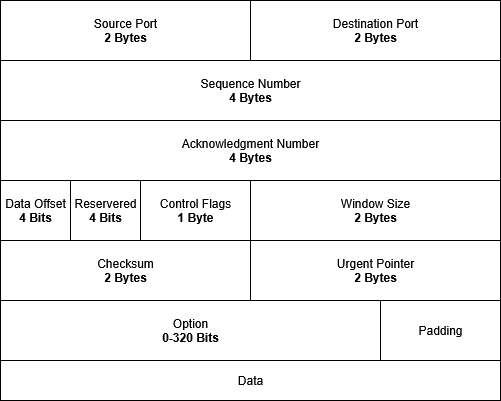
\includegraphics[alt={A block diagram of the TCP header format, detailing its fields and their sizes.}, height=8cm]{./images/tcp_header.png}
	\caption{The TCP header}
	\label{fig:tcp_header}
\end{figure}
The TCP header, figure~\ref{fig:tcp_header}, encodes the functionality of the TCP.
It follows the IP header in a datagram. The header is usually 20 bytes long, but
can be extended using options. It begins with the source and destination port, which
together with the source and destination addresses, are used to identify the connection.
The next two fields in the header are the sequence and acknowledgement numbers. The
sequence number is the sequence number of the first data byte in the data segment.
If the SYN flag is set the sequence number is referring to the initial sequence number
(ISN). The acknowledgement refers to the next sequence number the receiver is
expecting to receive, at the same time acknowledging that all sequence numbers
up to this point was received. Next is the data offset field, indicating where
the data begins. The reserved field following this must be 0. After this is the
1 byte flags field
\begin{itemize}
	\item \textbf{URG} Urgent pointer field is set
	\item \textbf{ACK} acknowledgement field is set
	\item \textbf{PSH} Push function, requesting that buffered data is sent immediately to the receiver
	\item \textbf{RST} Reset the connection
	\item \textbf{SYN} Synchronize sequence numbers
	\item \textbf{FIN} Sender is done sending data
\end{itemize}
The 2 byte window field specifies the number of bytes that may be in-flight at any one
time. This is the specified size of the sliding window that is used for flow
control purposes. Following the window field is a 2 byte checksum field, used for
detecting corruption of the TCP-header, data payload as well as a pseudo IP header,
containing information about the source and destination addresses, as well as the
protocol number and tcp packet length. In case the URG bit is set in the flags field,
the 2 byte urgent pointer header field indicates where the urgent data ends. Finally
the options field contains extension to the normal TCP header, containing among other, options
for maximum segment size and multipath TCP\cite{rfc8684}.

To ensure reliable delivery of TCP segments, each segment is assigned a sequence number.
This allows the receiver to reconstruct segments delivered out of order, and additionally
detect missing segments. The receiver sends acknowledgments, containing the next
expected sequence number, to signal to the sender that the data was successfully received.
The sequence number is a 32 bit number, with the initial sequence number (ISN)
selected randomly at the time when the TCP connection is established. This ensures that
sequence numbers from stale connections have a low probability of overlapping with
any active connection\cite{rfc793}.

The TCP connection is established via a three-way handshake. The client sends
a TCP packet with the SYN bit set in the flags field, this packet contains the
clients ISN. The server responds with a packet with the SYN and ACK bit set,
acknowledging the clients sequence number as well as providing the servers ISN.
Finally the client responds with an ACK, acknowledging the servers ISN. Following
this the client and server are synchronized, and communication may begin. A peer
may terminate its side of the connection by sending a FIN packet, signaling to
the other endpoint that one side has closed its side of the communication. The
closed endpoint may continue receiving data until the other endpoint also closes
it side\cite{rfc793}.
\subsubsection{User Datagram Protocol \label{UDP}}
\begin{figure}[b]
	\centering
	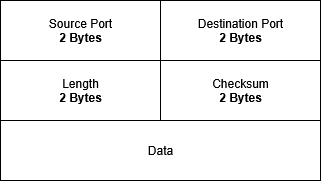
\includegraphics[alt={A block diagram of the UDP header format, detailing its fields and their sizes.}, height=4cm]{./images/udp_header.png}
	\caption{The UDP header}
	\label{fig:udp_header}
\end{figure}
The UDP, which was defined by RFC 768, is designed to
enable programs to transmit self-contained messages, know as datagrams, over a
packet-switched network. The UDP is designed to run on top of the IP\cite{rfc791},
using IP addresses and port numbers for addressing. The UDP is by design connectionless,
providing no guarantees for datagram delivery, duplicate datagrams or in-order
delivery. In exchange, the UDP aims to minimize the overhead present in the protocol.
As UDP is connectionless there is no need to establish a connection via a handshake,
instead datagrams can be transmitted directly, and they should be designed in
such a way that they can stand on their own. The UDP header, as seen in figure~\ref{fig:udp_header}
is only 8 bytes long,
consisting of the source and destination port, as well as the length of the datagram
and a checksum to verify the received datagram\cite{rfc768}. Even though UDP has
a checksum field its use varies depending on the implementation. Some implementations
may discard the datagram, or alternatively pass it along to the application with a 
warning, as UDP provides no way to recover from broken datagrams\cite{compute_rnetworking}. The minimal UDP
header (8 bytes) combined with the lack of a handshake makes UDP a protocol with
the bare minimum needed for datagram transfer.
Generally, UDP is used for applications where low latency is a requirement and some
amount of packet loss is deemed acceptable. It is then up to the application layer to
handle missing, reordered or duplicate datagrams.
\subsection{HTTP}

\subsection{Network Storage Protocols}


\clearpage

\section{QUIC}
\label{sec:quic}
The Internet's underlying infrastructure is in a state of constant evolution,
driven by a demand for decreased latency, increased throughput requirements and
a need for improved security. For many years now, the TCP has been the de-facto
solution for reliable and secure, when combined with Transport Layer Security (TLS), communications. However,
TCP was developed in a time where security and latency where not considerations,
at least not in the same way as in todays landscape. Over the years there have
been efforts to enhance TCP, such as multipath TCP\cite{rfc8684} and combining
TCP and TLS in HTTPS\cite{rfc2818} to improve security. This section of the thesis
will cover QUIC, a transport protocol developed to overcome the limitations and
improve the performance as compared to the TCP\cite{quic_transport_protocol_design}.

The importance of the QUIC protocol is not to be underestimated. It represents
a substantial change to the internet's transport layer, the first one in over
two decades. QUIC was initially developed by Google, and then later standardized
in RFC 9000\cite{rfc9000}. QUIC is designed to address the issues experienced
by TCP, with a focus on optimizing for web traffic. The main issues being the
Head-of-line (HOL) blocking, but also aiming to improve on other aspects,
such as integrating the TLS handshake into the transport handshake. A decision
that was made for QUIC specifically was to move the protocol out of the kernel
space and into the user space, allowing for rapid development and innovation\cite{quic_transport_protocol_design}.

This chapter of the thesis will outline the limitations of TCP that led to the
development of QUIC, give an overview of the architecture and logic that drives
QUIC.
\subsection{The motivation for a new transport protocol \label{quic_motivation}}
The TCP is a cornerstone of modern internet infrastructure. It has been a reliable
work horse for more than 40 years, ensuring communications between users and hosts
since its inception. However, as the design of TCP is largely colored by the
landscape when it was created, much of the improvements that have been made to TCP,
such as security, has had to be built on top of TCP, as these were not considerations
at the time of the TCP's inception. Todays internet landscape, with real-time content,
hyper mobile users and increased demands on latency, but also privacy and security, have exposed
some of the limitation imposed by the TCP stack. This section will outlined the
key issues that prompted the development of a new, modern protocol: QUIC.

\subsubsection{Head-of-Line Blocking}
The TCP guarantees that all frames will be delivered, reliably in-order. Seeing
as the TCP works as a single byte-stream the creates a phenomenon know as
Head-of-Line (HOL) blocking, where any lost packet will block the delivery of
all subsequent packets until the missing packet has been retransmitted. This
can potentially amplify issues in the network, increasing delays, decreasing
throughput and worsening the user experience. To combat this limitation, modern
network protocols, such as HTTP/2\cite{rfc9113}, have introduced measures to
combat the issue. HTTP/2 introduced multiplexing of multiple requests over one
connection, allowing multiple application-level streams, for example for different
resources such as images or javascript, to be multiplexed over a single TCP
connection. This means that HTTP/2 managed to mitigate application-level HOL
blocking, which was an issues in earlier versions of HTTP, it still potentially
suffered from transport level HOL blocking, as the multiplexed streams was still
sent over a single TCP connection. As a result a single lost packet in the TCP
stream still caused all other unrelated streams over the same connection to stall,
even if their packets were successfully delivered, until the offending packet
could be retransmitted. This in practice means that much of the improvements made
by HTTP/2 in this regard was negated by the issues of TCP, particularly in lossy
environments\cite{http2_vs_1}.

\subsubsection{Handshake Delay}
A limitation of the TCP stack is the delay caused by the TCP handshake. As discussed
in earlier chapters, establishing a TCP connection is done via a three-way handshake
(SYN, SYN-ACK, ACK). This handshake incurs one Round-Trip Time (RTT) of delay. In
addition, most application use TLS for security, and historically the TLS 1.2 handshake
and setup adds two additional RTTs of delay. While network bandwidth is ever increasing,
much of the communication done on the internet consist of short dialogues, that
are significantly impacted by the additional overhead brought on by the TCP plus TLS
handshake\cite{quic_transport_protocol_design}.

Some of the latency brought on by the TLS handshake is addressed by TLS 1.3, adding
support for 1-RTT and 0-RTT handshakes, at the cost of perfect forward secrecy\cite{rfc8446}. Even with
these enhancements, the TCP plus TLS handshake takes a minimum of 1,5 RTTs, due to the separation
of connection and security handshake.

\subsubsection{Protocol Ossification}
A big hurdle in deploying new protocols and extensions to existing ones on the internet,
is the protocol ossification of existing protocols on the internet. There exists a heap
of middleboxes, such as Network Address Translators (NATs) and firewalls that are
part of the network. These devices may be overly conservative, dropping or 
modifying packets that do not conform to their assumption. This is already an
issue for TCP enhancements, and entirely new protocols have no chance of reaching
their destination, without explicitly adding support in all necessary middleboxes.
To get around this, protocol designer have to design their protocols from the ground
up to be middlebox proof, such as QUIC encapsulating its protocol inside UDP as an
anti-ossification measure\cite{Ossification}.

A related issue of rolling out enhancements to existing protocols is that the
network stack tends to be part of the Operating System (OS) kernel. The networking
stack is tightly coupled to the OS, requiring OS updates or upgrades to implement
changes to existing protocols. With todays upgrade frequency it can take years
to roll out simple changes to the networking stack. QUIC moves the deployment of the 
protocol to the user space, improving the speed of development and deployment,
and opening up the space for multiple actors to create their own implementations of
the protocol\cite{quic_transport_protocol_design}.

\subsection{Background and evolution}
As discussed in Section \ref{quic_motivation}, the combinations of TCP, TLS and HTTP/2 are
plagued by issues that are difficult to circumvent without major overhauls or extensions to
the individual protocols, which due to protocol ossification is increasingly difficult. With
this in mind, a new protocol was being created, aiming to solve the issues of
HOL blocking, improved latency and circumventing protocol ossification. The answer
was the protocol that would later be standardized into QUIC, early on know as gQUIC.
QUIC began development back in 2012, by Jim Roskind, an engineer at google. Initially
the motivation for developing a new transport protocol was to improve support for
the now deprecated SPDY protocol\cite{googleQUICDesign}. QUIC was designed to run over
UDP, by encapsulating the protocol frames into UDP datagrams, and encrypting the contents,
the protocol could effectively sidestep the issues of middlebox interference, allowing
for rapid deployment without any necessary modifications to existing infrastructure.
To combat the issue of HOL blocking, QUIC implements transport level multiplexing of
data streams, allowing multiple independent streams to exist over one connection.
Packet loss in any of the data streams would not affect any of the other, blocking
only itself while waiting for retransmission. QUIC uses a combined connection and
cryptographic handshake, minimizing the latency of establishing a new connection.
While TCP uses IP-port tuples to identify connections, this does not allow for mobility
of the end user. If the IP or port of the user changes during the lifetime of the connection
the connection is dropped, and has to be reestablished. To combat this QUIC uses
Connection IDs to identify connections, allowing the connection to resume when
there is some change in network. QUIC was widely deployed on Google's front end servers,
and by 2017 it was already estimated that QUIC represented 7\% of global internet
traffic\cite{quic_transport_protocol_design}.

QUIC was submitted to the IETF for consideration in 2016, and a working group
was created for the purposes of standardizing QUIC. The goals of the working group
was to create a general purpose transport protocol that contained the benefits
of gQUIC. The custom cryptographic handshake was replaced with TLS 1.3, the packet header
was reworked into two types, a long and a short header, that was mostly encrypted
to prevent middlebox interference. Loss detection and congestion control mechanics
were updated, flow control semantics were separated into per stream and per connection
limits and version negotiation was introduced to enable future compatibility of the
protocol\cite{rfc9000}. In the end the protocol was standardized in a number of RFCs.
RFC 9000\cite{rfc9000} defines QUICs core transport mechanics, RFC 9001\cite{rfc9001} defines the use of TLS 1.3
and RFC 9002\cite{rfc9002} describes the loss detection and congestion control algorithms used by the
protocol. In addition, RFC 8999\cite{rfc8999} defines some version-independent
properties of QUIC, aligning QUICK packets, headers and versioning between
different versions of the protocol. Following the standardization the adoption
of QUIC has been quick. Chromium, and by extensions all chromium based browsers
has supported QUIC since before it was standardized\cite{chromium_quic}. Both
Firefox\cite{firefox_quic} and Safari\cite{safari_quic} added support for QUIC
soon after the standards were published. QUIC has shown the viability and potential
of deploying network protocols to the user space, enabling rapid adoption without
OS kernel updates.

\subsection{Architectural Overview}

The QUIC protocol is designed to be a general-purpose, secure and multiplexed
transport protocol, working on top of UDP. In comparison to TCP, which usually
is part of the OS kernel, QUIC is typically implemented in the user space, enabling
quick iteration and deployment of protocol enhancements. This section describes
QUIC's position in the networking stack, the different architectural parts and the
basic elements of the protocol's operation.

QUIC packets are directly encapsulate inside UDP datagrams. This design has both 
practical and implementation advantages. When deploying QUIC, the fact that the
wire image of QUIC packets are identical to that of UDP datagrams, means that they
pass seamlessly through middleboxes and firewalls, without suffering the adverse
effects of protocol ossification as is often the case in TCP. As discussed in Section \ref{UDP},
the UDP is a barebones protocol, with the minimum overhead needed to transmit datagrams. This
works to the advantage of the designer when building a protocol on top of UDP, as
the designer the freedom they need to implemnt their own semantics, withouth risking
interference from the underlying protocol. UDP provides the basic datagram services
that are then enhanced by the QUIC protocol, ensuring a secure, reliable and performant
protocol\cite{quic_transport_protocol_design}.

From an architectural perspective, QUIC incorporates three main layers, a transport
layer, a security layer and an application interface. From the bottom up, UDP provides
minimal mechanism for transmitting datagrams, withouth any guarantees. On top of this
QUIC implements its own transport layer, handling the multiplexing of datastreams,
ensuring reliable and in-order delivery of data as well as connection management
mechanics\cite{rfc9000}. QUIC security layer is fully integrated into the protocol, using TLS 1.3
for encryption of wire traffic, as well as authentication and authorization of peers, ensuring
secure communications between the endpoints. The security layer also protects most of
the packet headers, leaving only the necessary info for routing and version control
visible on the wire\cite{rfc9001}. The final layer exposes a standardized application
interface that can support virtually any application-layer protocol, the most prominent
one being HTTP/3\cite{rfc9113}.

One of the main innovation made by the QUIC protocol is the concept of transport-level,
mutiplexed and independent data streams. Any QUIC conneciton may contain one or multiple
data streams, seen entirely as their own independant object. This helps mitigate the
HOL blocking issues, as if the application is using multiple streams, when loss occurs,
only the stream on which the loss occured will be blocked. While the lossy stream is
blocking and waiting for retransmission, the other streams can continue sending as 
normal. QUIC uses per connection limits for the number of streams and per stream
flow control limits\cite{rfc9000}.

Connection management and and identification in QUIC differs in the IP-port tuple
combination that is tranditionally used in TCP. QUIC connection are identified by a
connection ID, which are independtly selected by the endpoints. The purpose of the
connection IDs is to allow the conneciton to survive changes in the network, for example
when a mobile users moves from a local network to cellular. The migration is done transparently
and securly, allowing the application to continue operations withouth interruption\cite{rfc9000}.

\subsection{Packet and Frame Structure}

QUIC packets are contained inside UDP datagrams, and together with the encryption
and integrity protection provided this gives a robust protection against protocol
ossification. As compared to TCP, where segmentation and reassembly of packets are
transparently done as part of the transport protocol and not accessible to the
application, QUIC defines a large set of different frames types for different,
distinct roles in conneciton establishments, data transfer and protocol logic
management. Depending on the packet type QUIC uses either a long header or short
header.
\begin{figure}[b]
	\centering
	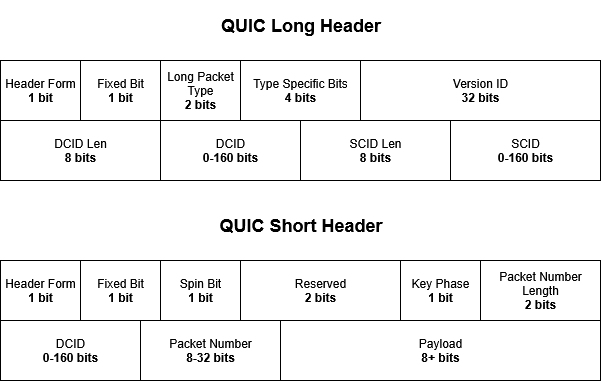
\includegraphics[alt={A block diagram of the QUIC short and long header format, detailing its fields and their sizes.}, height=8cm]{./images/quic_header.png}
	\caption{The QUIC header formats}
	\label{fig:quic_header}
\end{figure}

QUIC packets are divided into two general categories, those that use the long header
and those that use the short header. The long header is used during the establishment
phase of the connection, being used in the Version Negotation, Initial, 0-RTT, Handshake
and Retry packets. The long header, as seen in Figure~\ref{fig:quic_header}, contains the
necessary data for these function. The first bit of the long header is set to 1 to indicate
that this is a long header. The fixed bit following this is always set to 1, except
for Version Negotation packets. The Long Packet type indicates the type of packet,
and the 4 type specific bits are dependant on the packet type. Following this,
the version ID field indicates the specific QUIC version this packet is using, and
finally the destination and souce ID length and IDs contain the identifiers for
the source and destination of this packet. Following the header is, if relevant,
the specific packet type payload. In addition, the Initial, 0-RTT and Handshake
packet types includes a packet number length and packet number field. In comparison,
the short header is more compact, reducing per-packet overhead. The Header Form bit
(set to 0 in the short header case) and the Fixed bit is the same as for the long
header. The Spin Bit that follows may be used to make on path estimations of
the RTT. Following the two reserverd bits is the key phase bit, used to keep
track of the keys that are used to protect the packet. The packet number length
is the length of the packet number field minus one. Lastly is the destination ID
again indicating the recipient, the packet number used for protocols semantics
and finally the packet payload\cite{rfc9000}.

\begin{table}[tb]
	\centering
	\caption{Table of QUIC long header types}
	\label{tab:quic_long_header_types}
	\begin{tabular}{lll}
	\textbf{Packet Type}		  & \textbf{QUIC v1} & \textbf{QUIC v2} \\
	Initial   & 0x00    & 0b01    \\
	0-RTT     & 0x01    & 0b10    \\
	Handshake & 0x02    & 0b11    \\
	Retry     & 0x03    & 0b00   
	\end{tabular}
\end{table}
The long header packet type numbers differs between QUIC version 1 and version 2, as
is outline in Table~\ref{tab:quic_long_header_types}. Intial packets are used to initiate the connection and transmit
the initial TLS hanshake. The Handshake packet carries the subsequent
cryptographic messages, after the intial exchange. In case the connection attempt is
a resumption, the client may use the 0-RTT packe type to transmit encrypted application
data as part of the hanshake, basing the encryption on previously established keys. The
Retry packet type may be used by the server to force the client to
validate its address\cite{rfc9000}.

In QUIC there is only one short-header packet type, know as the 1-RTT packet. It is
used for the bulk of communication, taking advantage of the more compact short
header to reduce overhead on the connection, which is useful for high-throughput
applications. The header is in part protected by header protection, preventing
interference by middleboxes on the wire.

QUIC uses the concept of frames to enable protocol funcitonality. The payload of
QUIC packets consists of one or more frames, and the frames can be of different types,
enabling the transmission of application data and control data in the same packet. Frames
allow the QUIC protocol to signal transport events between the peers. Arguably the most
important frame type for data transmission is the STREAM frame. The stream frame
carries stream data associated with a specific stream. The STREAM frame contains
a stream identifier, byte offset and flags to track the state of the stream. The STREAM
frame implicitly creates a new stream in case the identifier is previously unknown.
The ACK frame is then used to acknowledge received packets. The ACK frame contains
one or more ranges of packet numbers that have been received, with possible gap values
indicating missing packets. This higher granularity enables the sender to only retransmit
the missing packets, lowering retransmission overhead in reordering scenarios. Other
important frame types include MAX\_DATA and MAX\_STREAM\_DATA for flow control
on the connection and stream level, PING frames to probe the peer and ensure that
the connection staus alive, CRYPTO frams for carrying TLS hanshake data and CONNECTION\_CLOSE
to terminate the connection. These are the most important frame types, with an
extensive list being available in RFC 9000 chapter 19 Frame Types and Formats. Together,
these frames allow for great control of transport functionality, allowing for explicit
control of the semantics\cite{rfc9000}.

\subsection{Streams}

The QUIC protocol is designed around the concept of streams. Streams are an abstraction
of a byte-streams, that are used to transmit data between applications. Streams may
be either bidirectional or unidirectional, that is, from the perspective of one peer,
the streams may be read-only, write-only or read and write. Any single connection may contain one or
more streams, with the streams being multiplexed and entirely indedependent from one
another. Streams are design to be lightweight, with minimal overhead. A stream can
open, closed and transmit data in a single frame, or alternatively the streams
can persist for longer lengths of time, up to the lifetime of the connection. The number
of streams and the amount of data that may be sent over a single stream is constrained
by the flow control. The different streams are identified via a unique identifier inside a connection,
the stream ID, which is a 62-bit integer. The reasoning for using a 62-bit integer is
that the two remaining bits are used to distinguish between unidirectional and bidirectional
streams, as well as identify the initiator of the stream, which may be either the
client or server\cite{rfc9000}.

The lifetime of a stream is explicitly managed by the peers. The stream is first
created by sending a stream frame, containing the stream ID of the stream that is
requested to be opened. Data transfer id done via STREAM frames, that carry the
application data that is to be transmitted. Once data transfer is complete, and
the application is done with the stream, it may be closed by sending a stream
frame with the FIN bit set, or alternatively send a RESET\_STREAM to abruptly end the
stream, signaling that no further data will be sent. On the receiver end the receiver
can read data from the stream, and may end the stream by sending a STOP\_SENDING frame,
signaling that no more data will be accepted on the stream\cite{rfc9000}.

The desing of QUIC streams is such that it directly addresses TCP's HoL blocking
issue. In TCP, the in-order delivery guarantee is implement on an entire connection,
resulting in the whole connection stalling in case of a lost packet until it is
retranmsitted and received. In comparison, QUIC building it's streams on top of
UDP, have implemented an in-order guarantee per stream. That is, any lost packet
only blocks the specific stream that packet belonged to, allowing the other streams
that may exists on the same connection to keep transmitting while the erronous
stream retransmits. This feature also works in the favor for control data,
as control frames is transmitted separately from the stream frames, they are not
affected by loss on any of the data streams\cite{rfc9000}. An example of this advantage
in action is in the HTTP/3 protocol. Here each client request is mapped to its own
bidirectional QUIC stream, and unidirectional streams are used for control and
push streams. HTTP/3 implementations should support at least 100 concurrent streams
taking advantage of the multiplexing afforded by QUIC\cite{rfc9114}. When a client
visits a web page, it may open tens of streams simultaneously, to fetch HTML, CSS,
JavaScript, images and font. If a packet containing part of an image is lost, QUIC
enables the HTML and CSS streams to continue delivering, improving render times
in lossy environments.

The lighweight desing of QUIC streams makes the suitable for short request-response
communications in other domains as well. DNS over QUIC takes advantage of the
stream semantics by creating a new QUIC stream for each request. Beside preventing
HoL blocking, DNS over QUIC takes advantage of QUIC's stream semantics by allowing
each DNS query to use a separate stream for communication. This allows the protocol
to cheaply process each request-response, forgoing the overhead of setting up a connection,
with its full handshake, instead creating a lightweight stream for the specific
communication. The multiplexed streams also allow the server to process and respond
to the queries out-of-order, allowing multiple, simoultaneous, outstanding queries
at any one time.

\subsection{Flow and Congestion Control}

To prevent fast senders or malicious actors from overwelming the receive buffer,
the QUIC protocol implements flow control on two levels, a per-stream flow limitation
and a per-conneciton limitation. The receiver controls the amount of data that can
be sent on any one QUIC stream at a time, as well as over the connection as a whole.
The receiver also limits the number of concurrent streams that the sender may open,
preventing the overwelming of the receiver with a large number of unique streams.
The limits are set during the hanshake process, but they may be updated by sending
MAX\_STREAM\_DATA and MAX\_DATA frames to signal that the flow control limits have
been increase. A receiver may not reduce the flow control limits during the connection.
If the sender is faster than the receiver it may reach a state where it is unable
to transmit data due to either one of the limit. In this case the sender should
send a STREAM\_DATA\_BLOCK or DATA\_BLOCK frame to signal to the receiver that
there is outstanding application data waiting to be sent, but it is currently unable
due to the flow control limits. Similarly the limit on the number of streams that
may be opened is set during the connectiion initialization phase. It may the layer be
increased by sending a MAX\_STREAMS frame, and similarly to the data flow control limits,
the streams limits may only be increased, not decreased. The sender can signal to the
receiver that it would like to open more streams by sending a STREAMS\_BLOCKED frame\cite{rfc9000}.
This granular control allows the protocol implementations to adapt the flow control
according to the environment, enabling improved performance especially in dynamic environments.

The QUIC protocol uses three different packet number spaces, separate for initial,
hanshake and application data spaces. This is as an effect of the fact that the
corresponding packets use different levels of encryption, ensuring that acknowledgements
sent in one packet number space does not cause retransmissions of packets of a different
encryption level. The packet numbers of QUIC are monotonically increasing, signaling
the order in which the packets were sent. That is, when retransmission occurs the
retransmitted packet uses the next available packet number instead of the same packet number.
To reconstruct reordered packets QUIC instead
uses a stream offset field inside the stream frames, to keep track of the correct
order of data. Loss detection in the QUIC protocol is then based on these packet
numbers. Loss can either be detected vi acknowledgement-based detection,
if a packet that is considered in-flight and is unacknowledged, but a packet
sent after the potential lost packet has been acknowledged, and enough time has passed
since the packet was sent. Alternatively, a Probe Timeout (PTO) causes one or two
datagrams to be sent out, expecting a response to test the reachability of the peer\cite{rfc9002}.

The QUIC protocol provides a set of generical signals that are design to support
multiple different sender-side congestion algorithms. A congestion algorithm similar
to TCP NewReno\cite{rfc6582} is outlined in RFC 9002. However, a sender is free to
choose any one algorithm they feel suits there use case, such as CUBIC, given that they conform
to the congestion control algorithms oulined in RFC 8085\cite{rfc8085}. One option
is to use QUIC packets which contain only ACK frames, as these do not count towards
the flow control limits, but the loss of these packets can be detected by the QUIC
algorithm\cite{rfc9002}.

The algorithm oulined in RFC 9002 begins in slow start, setting the initial congestion
window to 10 times the maximum datagram size. When in slow start the sender increases
the congestion number by the number of acknowledged bytes, until packet loss is detected. This
means that the congestion window can double every RTT as long as all inflight packets
are acknowledged. When packet loss is detected the sender enters recovery period.
During the recovery period the congestion windows is reduced to half its currently
size, and this reduction may be done instantly when entering the recovery period
or gradually using some other mechanism. Any additional detect loss during this
period does not affect the congestion window size. The recovery period ends once
the congestion window has been reduced to the new size, and the sender has sent
a packet and that packet has been acknowledged. From here the sender enters congestion 
avoidance. During the congestion avoidance period, the sender may at maximum increase
the congestion window by one maximum datagram size for each complete congestion
window that has been acknowledged. In case loss is detected the sender goes back
into recovery mode. In case persisent congestion is detected, that is the continuous
loss of all sent packets, the sender reenters slow start mode, and the process
starts over\cite{rfc9002}.

In the QUIC algorithm there may be a situation where reordering of packets causes
the receiver to receiver packets to which it does not have the necessary keys to
decrypt, such as handshake or 0-RTT packets arriving before the initial packets.
Loss of these packets may be ignored, unless an earlier packet from the same packet space
has been acknowledged, in which case the loss must not be ignored. When a probe
packet is sent it should not be blocked by the congestion cnotrller, even if they might exceed the current
congestion, and these packet should also be accounted for as being in-flight. The
sender should pace the sending of its packets, as large bursts of packets may induce 
congestion or packet loss. A lack of application data or pacing on the part of the
sender may cause the congestion window to be underutilized. In this case the congestion
window should not be increased\cite{rfc9002}.

\subsection{Connections}

The QUIC protocol is a stateful, connection-oriented protocol where the QUIC
connection functions as the shared state between peers. Connections are created
via a handshake, during which both the transport and security hanshake is performed,
with the security handshake being based in TLS 1.3\cite{rfc9001}. The handshake establishes
the connection, and the parameters for the connection are declared. The parameters
are individually decided by the peers, and the opposite peer needs to comply with
the conditions set. It is possible via 0-RTT data transfer to transfer application
data as part of the initial message, before the server has responded, and the server
may already start sending data before the final hanshake message from the client.
This allows the protocol to exchange some security guarantess for improved latency
when establishing a connection\cite{rfc9000}.

\subsubsection{Connections and Identifiers}

From a connection standpoint one of the innovations made by the QUIC protocol, as
compared to TCP, which uses port-IP tuples to identify connections, is the Introduction
of connection IDs. The point of connection IDs is to make the protocol more resilient
to changes in the lower level protocols, such as IP addresses changing when a client
moves from one network to another. In case of connection migration from one network to
another the connection ID used is also changed at the same time. This is to prevent
passive listener from tracking a peer from one network to another, which could be
done via correlating connection IDs\cite{rfc9000}.

In a QUIC connection each peer decides the connection ID for the other peer. Initially
the connection IDs are issued during the handshake phase, and the connection ID is
associated with a sequence nubmer, starting from 0. A peer may use NEW\_CONNECTION\_ID frames
to assign a new connection ID to its peer, at the same time increasing the sequence
number by one. A peer can and should issue multiple connection IDs to its other peers,
and should accept packets originating from any of these connection IDs. This give the peer
a sufficient number of unused connection IDs that are available for later use during
the connection. Packets from the assigned connection IDs should be accepted until
they are explicitly retired, either using a RETIRE\_CONNECTION\_ID frame or by
sending a NEW\_CONNECTION\_ID fram with the Retire Prior To value increased, which
forces the peer to retire the related connection IDs. Sending a RETIRE\_CONNECTION\_ID
frame implicitly requests the peer to issue a new connection ID to replace the one
that has just been removed. A connection ID must not be retired withouth alerting the peer,
and the number of connection IDs that have been locally retired, that is the connection
ID is retired and a RETIRE\_CONNECTION\_ID fram has been sent, but no acknowledgement
has yet been received, should be kept to a limited number\cite{rfc9000}.

When a QUIC packet is received it is attempted to match this packet to an existing
connection. If the recepient is a server it is also possible that the incoming
packet is part of a new connection. If it is not possible to associate the packet
with any connectino ID of any existing connection, and the packet is not part of
initializing a new connection, then a Stateless Reset may be sent in response. If
a packet is received, but it is not consistant with the connection, the packets
are discarded. Such a scenario could be incorrect versioning or inability to
decrypt the packet\cite{rfc9000}.

\clearpage

\section{The Server Message Block protocol}
\label{sec:smb}
\subsection{Information about the SMB protocol}
\clearpage
\section{Implementing QUIC as transport for SMB server}
\label{sec:implementation}
\subsection{MsQuic architecture and API}

\subsection{Fusion SMB server QUIC transport layer design}
\clearpage
\section{Performance and interoperability benchmarking}
\label{sec:benchmark}
\subsection{Test environment}

\subsubsection{Hardware environment}

\subsubsection{SMB over QUIC implementations analyzed}

\paragraph{Windows SMB client/server}

\paragraph{Fusion SMB server}

\subsection{Test scenarios}

\subsubsection{interoperability tests}

\subsubsection{Becnhmarking workloads}

\subsection{Results}
\clearpage
\section{Conclusions}
\label{sec:conclusion}
\label{sec:summary}

\subsection{Discussion}

\subsection{Future work}

\clearpage
%% Bibliography/ list of references
%%
%%\nocite{*} % print uncited references in the bibliography
\printbibliography[heading=bibintoc] %, add the title to the table of conten

\end{document}
